\documentclass[aspectratio=169, pdf, 8pt, unicode]{beamer}
\usepackage[american,russian]{babel}
\usepackage[default]{sourcesanspro}
\usepackage{float}
\usepackage{graphicx}
\usepackage{pgfplotstable}
\usepackage{caption}
\usepackage{amsmath}
\usepackage{amssymb}
\usepackage{setspace}
\usepackage{fancyvrb}
\usepackage[outputdir=aux]{minted}
\usepackage{url}

\DeclareCaptionLabelFormat{gostfigure}{Рисунок #2}
\captionsetup[table]{labelsep=endash,justification=justified,singlelinecheck=false,font=normalsize,skip=0pt} 
\captionsetup[figure]{labelformat=gostfigure,labelsep=endash,justification=centering,singlelinecheck=false,font=normalsize} 
\pgfplotsset{compat=1.9}

\mode<presentation> {
\usetheme{Madrid}
}

\setbeamerfont{institute}{size=\normalsize}
\setbeamertemplate{itemize/enumerate body begin}{\large}
\setbeamertemplate{itemize/enumerate subbody begin}{\tiny}

\title[Теория и практика многопоточного программирования]{Теория и практика многопоточного программирования}

\author{Неганов Алексей}

\institute[МФТИ]{
    Московский физико-технический институт (национальный исследовательский университет)\\
    Кафедра теоретической и прикладной информатики\\
}

\date{Москва 2020}

\setbeamertemplate{caption}[numbered]

\begin{document}

\begin{frame}
\titlepage
\end{frame}

\begin{frame}
\frametitle{Вспомним теорию}
Виды синхронизации:
\begin{itemize}
\item Coarse-grained
\item Fine-grained
\item Optimistic
\item Lazy
\item Nonblocking
\end{itemize}
Корректность алгоритма:
\begin{itemize}
\item Инварианты
\item Линеаризуемость
\end{itemize}
\end{frame}

\begin{frame}[fragile]
\frametitle{Flat combining}
\begin{figure}[H]
\begin{minipage}{0.8\textwidth}
\begin{verbatim}
template <class T> class LockStack {
    std::stack<T *> m_Stack;
    std::mutex      m_Mutex; 
public:
    void push( T& v ) {
        m_Mutex.lock();
        m_Stack.push( &v );
        m_Mutex.unlock();
    }
    T * pop() {
        m_Mutex.lock();
        T * pv = m_Stack.top();
        m_Stack.pop()
        m_Mutex.unlock();
        return pv;
    }
};
\end{verbatim}
\end{minipage}
\end{figure}
\end{frame}

\begin{frame}[fragile]
\frametitle{Flat combining}
\begin{figure}[H]
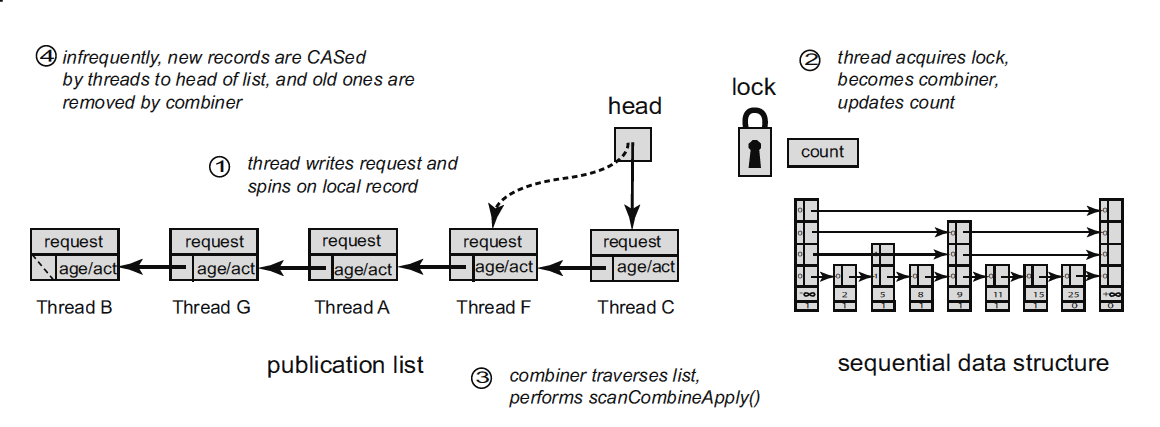
\includegraphics[width=0.9\textwidth]{fig/flat_combining.png}
\end{figure}
\url{https://www.cs.bgu.ac.il/~hendlerd/papers/flat-combining.pdf}
\end{frame}

\begin{frame}[fragile]
\frametitle{Lock-free stack}
\begin{figure}[H]
\begin{minipage}{0.8\textwidth}
\begin{verbatim}
template<typename T> class lock_free_stack {
struct node {
    T data;
    node* next;
    node(T const& data_): data(data_) {}
};
std::atomic<node*> head;
public:
    void push(T const& data) {
        node* const new_node=new node(data);
        new_node->next=head.load();
        while(!head.compare_exchange_weak(new_node->next,new_node));
    }
};
\end{verbatim}
\end{minipage}
\end{figure}
\end{frame}

\begin{frame}[fragile]
\frametitle{Lock-free stack: ABA}
\begin{figure}[H]
\begin{minipage}{0.8\textwidth}
\begin{verbatim}
void simple_pop(T& result) {
    node *old_head=head.load();
    while(!head.compare_exchange_weak(old_head, old_head->next));
    result=old_head->data;
}
\end{verbatim}
\end{minipage}
\end{figure}
\end{frame}

\begin{frame}[fragile]
\frametitle{Lock-free stack: free list}
\begin{figure}[H]
\begin{minipage}{0.8\textwidth}
\begin{verbatim}
template<typename T> class lock_free_stack {
    std::atomic<unsigned> threads_in_pop;
    std::atomic<node*> to_be_deleted;
    void try_reclaim(node* old_head);
public:
    std::shared_ptr<T> pop() {
        ++threads_in_pop;
        node* old_head=head.load();
        while(old_head && !head.compare_exchange_weak(old_head, old_head->next));
        std::shared_ptr<T> res;
        if(old_head)
            res.swap(old_head->data);
        try_reclaim(old_head);
        return res;
    }
};
\end{verbatim}
\end{minipage}
\end{figure}
\end{frame}

\begin{frame}[fragile]
\frametitle{Lock-free stack: hazard pointers}
\begin{figure}[H]
\begin{minipage}{0.8\textwidth}
\small
\begin{verbatim}
std::shared_ptr<T> pop() {
    std::atomic<void*>& hp=get_hazard_pointer_for_current_thread();
    node *old_head=head.load();
    do {
        node *temp;
        do {
            temp = old_head;
            hp.store(old_head);
            old_head=head.load();
        } while(old_head!=temp);
    } while(old_head && !head.compare_exchange_strong(old_head,old_head->next));
    hp.store(nullptr);
    std::shared_ptr<T> res;
    if(old_head) {
        res.swap(old_head->data);
        if(outstanding_hazard_pointers_for(old_head))
            reclaim_later(old_head);
        else
            delete old_head;
        delete_nodes_with_no_hazards();
    }
    return res;
}
\end{verbatim}
\end{minipage}
\end{figure}
\end{frame}

\begin{frame}[fragile]
\frametitle{Lock-free stack: backoff}
\begin{figure}[H]
\begin{minipage}{0.8\textwidth}
\small
\begin{verbatim}
void push(T const& data) {
    node *const new_node=new node(data);
    node *t = head.load(std::memory_order_relaxed);
    while (1) {
        new_node->next.store(t, std::memory_order_relaxed);
        if (head.compare_exchange_weak(t, new_node, std::memory_order_release, std::memory_order_relaxed))
           return;
        bkoff();
    }
}

node *pop() {
   typename gc::Guard guard; // Hazard pointer guard
   while (1) {
      node *t = guard.protect(head);
      if ( t == nullptr )
         return nullptr ;  // stack is empty

      node *pNext = t->next.load(std::memory_order_relaxed);
      if ( head.compare_exchange_weak(t, pNext, std::memory_order_acquire, std::memory_order_relaxed ))
           return t;
      bkoff();
   }
}
\end{verbatim}
\end{minipage}
\end{figure}
\end{frame}

\begin{frame}[fragile]
\frametitle{Elimination backoff}
\begin{figure}[H]
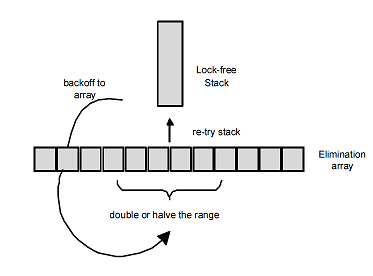
\includegraphics[width=0.5\textwidth]{fig/elimination_backoff_1.png}
\end{figure}
\end{frame}

\begin{frame}[fragile]
\frametitle{Elimination backoff}
\begin{figure}[H]
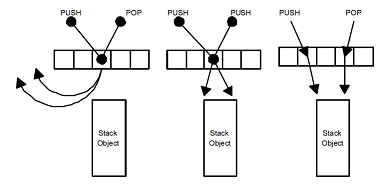
\includegraphics[width=0.5\textwidth]{fig/elimination_backoff_2.png}
\end{figure}
\end{frame}

\end{document}
